\documentclass{beamer}
%\usetheme{Hannover}


\usepackage{verbatim}
\usepackage{fancyvrb}
\usepackage{colortbl}
\usepackage{caption}
\usepackage{subcaption}
\usepackage{multicol}
\usepackage{amsfonts}
\usepackage{mathtools}
\usepackage{changepage}
\usepackage{gensymb}
\usepackage{csquotes}
\usepackage{float}
\usepackage{listings}
\usepackage{amssymb}
\usepackage{amsthm}
\usepackage{amsmath}
\usepackage[utf8]{inputenc}
\usepackage{csquotes}
\usepackage{graphicx}
\usepackage[english]{babel}
\usepackage[
	backend=bibtex,
	style=authoryear,
	citestyle=authoryear
]{biblatex}
\addbibresource{~/.config/assets/LaTeX/auni.bib}

\setboolean{@twoside}{false}
\setlength{\parskip}{1em}
\setlength{\parindent}{4em}
\renewcommand{\baselinestretch}{1}
\makeatletter
\renewcommand{\@seccntformat}[1]{}
\makeatother

\theoremstyle{definition}
\newtheorem{exmp}{Example}[section]

\author{Chris Sobczak}
\title{Operating System Survey of Public Domains}
\subtitle{Identifying Market Share Breakdown}
\institute{Simon Fraser University}
\date{\today}

\setbeamertemplate{itemize subitem}[circle]



\begin{document}


\begin{frame}
\titlepage
\end{frame}



\begin{frame}
\frametitle{This Survey}
\begin{itemize}
\item Sampling public websites to determine the operating system used to run the site
\end{itemize}

\begin{figure}[htp]
\centering

\includegraphics[width=.2\textwidth]{graphics/windows.png}\quad

\includegraphics[width=.2\textwidth]{graphics/linux.png}

\medskip


\includegraphics[width=.2\textwidth]{graphics/redhat.png}\quad

\includegraphics[width=.2\textwidth]{graphics/debian.png}\quad

\includegraphics[width=.2\textwidth]{graphics/freebsd.png}\quad

\includegraphics[width=.2\textwidth]{graphics/puffy.png}
\end{figure}
\end{frame}



\begin{frame}
\frametitle{Questions}

\begin{columns}
\begin{column}{0.4\textwidth}
\begin{itemize}
\item What operating system (OS) do most websites run?
\item Do certain categories of sites more often run one OS compared to other categories?
\item What other info might we get from these machines (services running, nginx v. Apache)?
\end{itemize}
\end{column}
\begin{column}{0.8\textwidth}
\begin{figure}
\centering
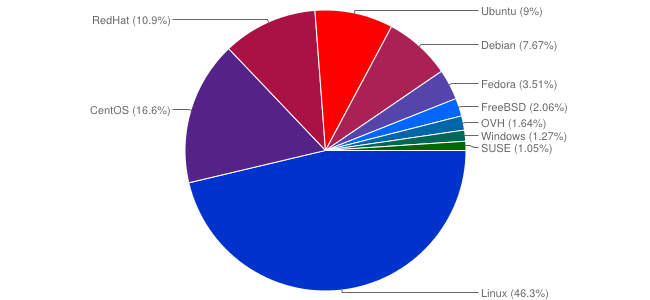
\includegraphics[scale=0.4]{graphics/market.png}
\caption{\cite{solvedns}}
\end{figure}
\end{column}
\end{columns}
\end{frame}





\begin{frame}
\frametitle{Problem With Current Numbers}

\begin{itemize}
\item Most of the statistics about operating system market share
of servers is by:
\begin{itemize}
\item The number of downloads from the vendor's website
\item Self reported counting during the install
\item Self reporting by domain owners
\end{itemize}

\end{itemize}

\centering
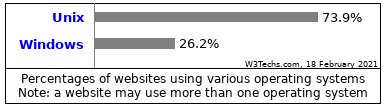
\includegraphics[scale=0.75]{graphics/w3tech.png}
\end{frame}


\begin{frame}
\frametitle{Purpose}
\begin{itemize}
\item Will a survey validate the self reported statistics?
\item Are open source server OSs under-reported since it is harder to count these machines (\cite{venkris2012})?
\end{itemize}
\centering
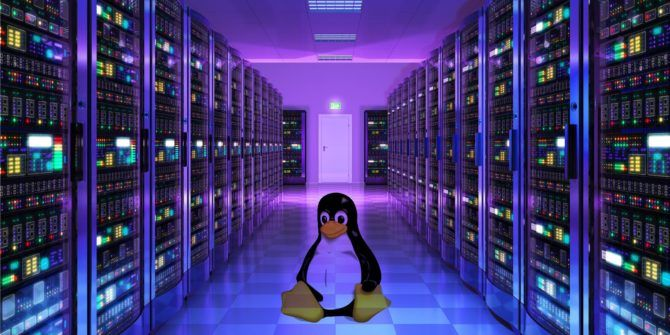
\includegraphics[scale=.45]{graphics/server.jpg}
\end{frame}




\begin{frame}
\frametitle{Outline}
\begin{itemize}
\item Target Population: The entire internet (all public facing web servers)
\item Sampling Frame: Index of all public facing domains that have content (using domain registrars)
\item Sampling Unit: Domain
\item Observational Unit: The physical computer/server
\end{itemize}
\end{frame}


\begin{frame}
\frametitle{References}
\printbibliography
\end{frame}

\end{document}
